\section{Balkar}

\paragraph{Elastisk vridning}
Antag att man har en stång med cirkulärt tvärsnitt fäst i ena ändan som man vrider med ett moment $M_{\text{v}}$ (i varje ända). Detta ger en vinkeldeformation $\theta$ i det yttersta tvärsnittet och $\gamma$ relativt linjen parallellt med stångens riktning. Om stången har en längd $l$ och en radius $a$, ger detta
\begin{align*}
	L\gamma = a\theta.
\end{align*}
Kombinerad med resultatet från delen om skjuvspänning ger detta
\begin{align*}
	\frac{\theta}{L} = \frac{\tau}{G}.
\end{align*}
Antag nu att $\tau = \frac{M_{\text{v}}}{K}$. Detta ger
\begin{align*}
	\frac{\theta}{L} = \frac{M_{\text{v}}}{GK}.
\end{align*}
$K$ är en konstant som beror av stångens geometri.

Hur beräknar vi $K$? Jo, man integrerar momentets differential över tvärsnittet. Vi vet att detta differentialet ges av kraft gånger arm, och det är så skjuvspänningen kommer in.

\paragraph{Balkböjning - fundamentala koncept}
För att beskriva balkar behöver vi införa fler olika sorters inre krafter och moment. Dessa illustreras i figur \ref{fig:beam_forces}.
\begin{figure}[!ht]
	\centering
	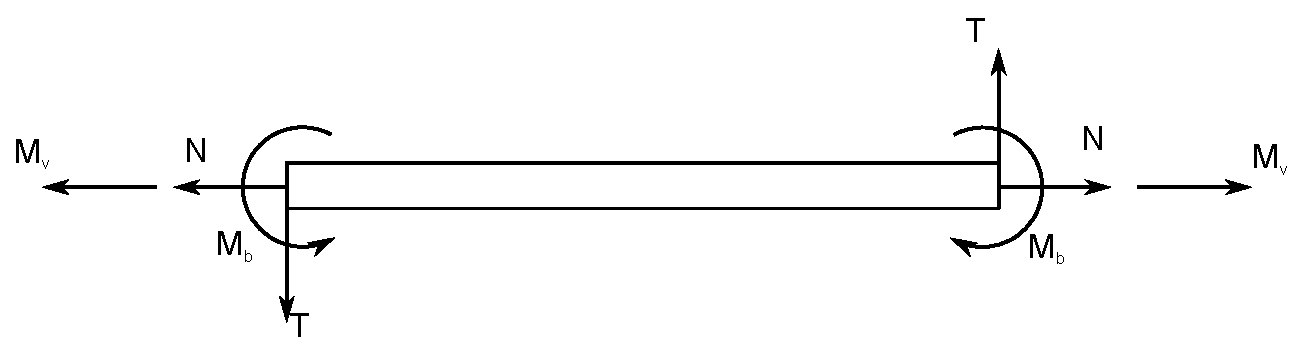
\includegraphics[width = 0.5\textwidth]{./Images/beam_forces.eps}
	\caption{Illustration av inre krafter och moment i en balk.}
	\label{fig:beam_forces}
\end{figure}
Vi har infört normalkraften $N$, tvärkraften $T$, det böjande momentet $M_{\text{b}}$ och det vridande momentet $M_{\text{v}}$.

Låt $u$ vara balkens deformation normalt på dens utsträkning. Vi har från enaxliga tillståndet att
\begin{align*}
	\frac{\Delta u}{L} = \frac{N}{EA}.
\end{align*}
Låt $\theta$ och $\phi$ vara vinklarna för böjning och vridning. Vi har från innan att
\begin{align*}
	\frac{\Delta\theta}{L} = \frac{M_{\text{v}}}{GK},
	\frac{\Delta\phi}{L} = \frac{M_{\text{b}}}{EI}.
\end{align*}

\paragraph{Allmänt tillstånd för en balk}
Snitta nu ut ett element med längd $\dd{x}$ från en balk. Om balken påverkas av en last $q$ per längdenhet, ger kraftjämvikten
\begin{align*}
	T(x + \dd{x}) - T(x) + q(x)\dd{x} = 0,
\end{align*}
vilket ger
\begin{align*}
	\dv{T}{x} = -q.
\end{align*}
Momentjämvikt kring centrum ger
\begin{align*}
	M(x + \dd{x}) - M(x) - (T(x) + T(x + \dd{x}))\dd{x} = 0.
\end{align*}
Bidraget från tvärkraften ges av
\begin{align*}
	T(x) + T(x + \dd{x}) &= 2T(x) + \dv{T}{x}\dd{x} \\
	                     &= 2T(x) - q(x)\dd{x}.
\end{align*}
Insatt i momentjämvikten fås
\begin{align*}
	M(x + \dd{x}) - M(x) - \frac{1}{2}\dd{x}(T(x) + T(x + \dd{x})) = M(x + \dd{x}) - M(x) - T(x)\dd{x} + \frac{1}{2}\dd{x}q(x)\dd{x}.
\end{align*}
Vi försummar nu alla andra ordningens termer, vilket ger
\begin{align*}
	\dv{M}{x} = T.
\end{align*}
Kombinerat med det förra resultatet fås
\begin{align*}
	\dv[2]{M}{x} = -q.
\end{align*}

\paragraph{Randvillkor för balkar}
En balk kan i en given ända vara
\begin{itemize}
	\item fri, vilket ger $T = 0$ och $M = 0$.
	\item fritt upplagd, vilket ger $M = 0$.
	\item glidinspänd, vilket ger $T = 0$.
	\item fast inspänd, vilket ej ger villkor för de inre krafterna och momenterna.
\end{itemize}

\paragraph{Balkböjning vid normalspänning}
Vid böjning inför vi en $z$-koordinat normal på medellinjen genom balken, och centrerar våra koordinater i tvärsnittets tyngdpunkt. Vi antar till att börja med att tvärsnittet är symmetrisk med avseende på $z$-axeln, samt att
\begin{itemize}
	\item plana tvärsnitt förblir plana.
	\item tvärsnitt förblir vinkelräta mot medellinjen.
	\item det för varje $z$ är ett enaxligt samband mellan $\sigma$ och $\varepsilon$.
	\item alla deformationer är små och för balkar vars längd är mycket större än deras tjocklek.
\end{itemize}
De två första uppfylls om skjuvspänningen är försumbar jämförd med normalspänningen.

Betrakta nu ett litet element med ursprunglig längd $L_{0}$ vars medellinje har böjts så den har krökningsradie $R$. Geometri ger oss
\begin{align*}
	(R + z)\phi = L_{0}(1 + \varepsilon(z)).
\end{align*}
I $z = 0$ har vi
\begin{align*}
	R\phi = L_{0}(1 + \varepsilon_{0}),
\end{align*}
vilket ger
\begin{align*}
	L_{0}(1 + \varepsilon_{0}) + z\phi &= L_{0}(1 + \varepsilon(z)), \\
	\varepsilon(z)                     &= \varepsilon_{0} + \frac{\phi}{L_{0}}z.
\end{align*}
Vi kan även substituera för $\phi$ för att få
\begin{align*}
	\varepsilon(z) = \varepsilon_{0} + \frac{1 + \varepsilon_{0}}{R}z.
\end{align*}

Om vi snittar och får någon given normalkraft $N$ på ytan, gäller det att
\begin{align*}
	N &= \integ{A}{}{F}{} \\
	  &= \integ{A}{}{A}{\sigma}.
\end{align*}
Hookes lag ger
\begin{align*}
	N &= \integ{A}{}{A}{E\left(\varepsilon_{0} + \frac{z}{R}\right)} \\
	  &= \integ{A}{}{A}{E\varepsilon_{0} + E\frac{z}{R}}.
\end{align*}
Om vi antar att elasticitetsmodulen är konstant över ytan, kan vi dra ut konstanter. Den andra integralen är då tyngdpunktens $z$-koordinat (om vi antar homogen massfördelning), som per definition var $0$. Detta ger
\begin{align*}
	N = E\varepsilon_{0}A.
\end{align*}

Vi beräknar vidare det böjande momentet $M_{y}$, som är normalt på både längdriktningen och $z$-koordinaten. Detta ges av
\begin{align*}
	M_{y} &= \integ{A}{}{A}{\sigma z} \\
	      &= \integ{A}{}{A}{Ez\left(\varepsilon_{0} + \frac{z}{R}\right)} \\
	      &= \integ{A}{}{A}{Ez\varepsilon_{0} + \frac{E}{R}z^{2}}.
\end{align*}
Första integralen är igen lika med $0$. Andra är relaterad till yttröghetsmomentet
\begin{align*}
	I_{y} = \integ{A}{}{A}{z^{2}}.
\end{align*}
Vi får alltså
\begin{align*}
	M_{y} = \frac{EI_{y}}{R}.
\end{align*}
Vi kan nu sätta ihop dessa resultat och få
\begin{align*}
	\sigma = \frac{N}{A} + \frac{M_{y}}{I_{y}}z.
\end{align*}

Vid ren böjning, dvs. ingen normalkraft, kan vi skriva
\begin{align*}
	\abs{\sigma}_{\text{max}} = \frac{\abs{M_{y}}\abs{z}_{\text{max}}}{I_{y}}.
\end{align*}
Vi kan införa böjmotståndet
\begin{align*}
	W_{\text{b}} = \frac{I_{y}}{\abs{z}_{\text{max}}},
\end{align*}
och får då
\begin{align*}
	\abs{\sigma}_{\text{max}} = \frac{\abs{M_{y}}}{W_{\text{b}}}.
\end{align*}

\paragraph{Allmänt tillstånd för en balk}
Vi försöker nu sammanställa dessa resultat till ett allmänt tillstånd för balken.

Geometri ger oss att
\begin{align*}
	\frac{1}{\abs{R}} = \frac{\dv[2]{u}{x}}{\left(1 + \left(\dv{u}{x}\right)^{2}\right)^{\frac{3}{2}}}.
\end{align*}
För små deformationen är derivatan mycket liten. Om vi definierar positiv krökning som att balken kröks nedåt, fås
\begin{align*}
	\frac{1}{R} = -\dv[2]{u}{x}.
\end{align*}
Materialsamband ger
\begin{align*}
	M_{\text{b}} = -EI_{y}\dv[2]{u}{x}.
\end{align*}
Vi har även
\begin{align*}
	\dv[2]{M_{\text{b}}}{x} = -q,
\end{align*}
vilket slutligen ger
\begin{align*}
	\dv[2]{x}\left(EI_{y}\dv[2]{u}{x}\right) = q.
\end{align*}

Till detta tillståndet hör olika sorters randvillkor. Några enkla varianter av randvillkor är
\begin{itemize}
	\item $u$ eller $T$ givna i ändpunkterna.
	\item $\dv{u}{x}$ eller $M$ givna i ändpunkterna.
\end{itemize}
Vi kan även karakterisera ändpunkter som
\begin{itemize}
	\item fria, dvs. $T = 0$ och $M = 0$.
	\item fritt upplaggda, dvs. $u = 0$ och $M = 0$.
	\item fast inspända, dvs. $u = 0$ och $\dv{u}{x} = 0$.
	\item glidande inspända, dvs. $\dv{u}{x} = 0$ och $T = 0$.
\end{itemize}

\paragraph{Superposition}
Balkens allmänna tillstånd är linjärt, så om man har någon komplicerad sammansättning av yttre laster och krafter, kan man separera problemet i olika delproblem, lösa de separat och superponera lösningen.

\paragraph{Plasticering av balk}
Betrakta en balk som endast utsätts för ett böjmoment $M$. Vid inledande plasticering är
\begin{align*}
	\sigma_{\text{max}} = \sigma_{\text{s}}.
\end{align*}
Vi vet i detta fallet att
\begin{align*}
	\sigma_{\text{max}} = \frac{\abs{M}}{W_{\text{b}}},
\end{align*}
vilket ger
\begin{align*}
	M_{\text{s}} = W_{\text{b}}\sigma_{\text{s}}.
\end{align*}

Vid full plasticering är spänningen lika med $\sigma_{\text{s}}$ i hela balken. Från detta kan man beräkna böjmomentet. Som ett exempel fås för ett rektangulärt tvärsnitt som böjs i höjdriktning:
\begin{align*}
	M_{\text{f}} = 2\cdot\sigma_{\text{s}}b\frac{h}{2}\cdot\frac{h}{4}.
\end{align*}
Man kan även visa att detta är lika med $\frac{3}{2}M_{\text{s}}$.

Vid avlastning kan man använda superposition för att få spänningstillståndet. Det kommer visa sig att restspänningen är diskontinuerlig i mitten.

\paragraph{Tillstånd för axialbelastad balk}
Betrakta en balk som utsätts för en axial belastning, och snitta ut ett element i den enligt figur \ref{fig:skew_beam_forces}.
\begin{figure}
	\centering
	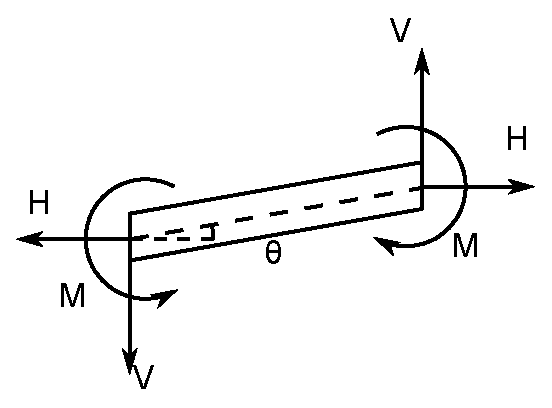
\includegraphics[width = 0.5\textwidth]{./Images/skew_beam_forces.eps}
	\caption{Snitt i en axialbelastad balk, där snittet görs vertikalt relativt det odeformerade läget.}
	\label{fig:skew_beam_forces}
\end{figure}
Kraft- och momentjämvikter ger
\begin{align*}
	V(x + \dd{x}) - V(x) + q\dd{x} = 0, \\
	H(x + \dd{x}) - H(x) = 0, \\
	M(x + \dd{x}) - M(x) - V(x)\dd{x} + H\dv{w}{x}\dd{x} = 0,
\end{align*}
där vi har utnyttjat att vinkeln $\theta$ ges av derivatan av utböjningen och försummat det andra ordningens bidraget till momentet från den utbrädda lasten. Detta ger
\begin{align*}
	\dv{V}{x} = -q,\ \dv{H}{x} = 0,\ \dv{M}{x} = V - H\dv{w}{x}.
\end{align*}
Man kan visa att till första ordningen är $H = N$, och $N$ ges av den yttre axiala lasten (och eventuella volymkrafter). Kombinationen av dessa ekvationer ger då
\begin{align*}
	\dv[2]{x}\left(EI\dv[2]{w}{x}\right) - N\dv[2]{w}{x} = 0.
\end{align*}